\subsection{The Nature of Human Actions}
\label{sec:gote}
Jeoroen Kraaijenbrink has made a paper on the entrepreneurial process\todo{cite here}. The focuses on the dimensions of the different models rather than the models themselves, as well as a suggestion on connection the nature of entrepreneurship with the nature of human actions. The connection to the human actions is mostly a suggestions, with a few relations to how the human actions are biased. We bring a suggestion to an extended version of this model, combining the model with a cognitive process.

\subsubsection*{GOTE}
G.O.T.E. is an acronym created by Robert Cohen and a method used in theatre and drama\todo{cite here}. The method is normally used for reminding the actor of four elements needed when creating a character and its situation. The acronym is for \emph{Goal}, \emph{Obstacle}, \emph{Tactics} and \emph{Expectations}. The goal is what the character desires, the obstacle is what hinders the character in achieving the goal, the tactic is the method used to achieve goals, and the expectation is what the character expects to achieve if succeeding. We believe the method is also suitable for entrepreneurship to create a ends-driven model based on methods rather than specific models.

The GOTE can be used to describe processes in entrepreneurship on a high level, as seen on \figref{fig:gote}. The ultimate goal is to create a product or a service. Several obstacles stands in the way, which are found through existing models, such as Porter's Five Forces. The tactics are a list of ways to overcome the obstacles. The expectations of the goal is often to gain money, although it sometimes is for the thrill of the process and satisfaction in seeing the end goal.

\begin{figure}
\begin{center}
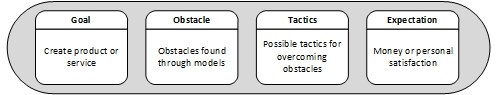
\includegraphics[scale=0.7]{./pics/gote}
\caption{The GOTE method used in entrepreneurship on high level}
\label{fig:gote}
\end{center}
\end{figure}

An interesting take on the GOTE method is the fact that it works on several layers, in both acting and entrepreneurship. This means using the tactics as a new goal, and finding obstacles and tactics for this goal. The expectation for the goal is to come closer to the upper level goal. An example for this in relation to our project can be seen in \figref{fig:gote_watchr}.


\begin{figure}
\begin{center}
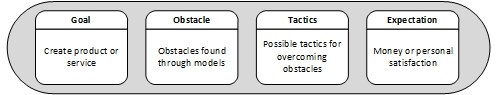
\includegraphics[scale=0.7]{./pics/gote}
\caption{The GOTE method used several layers for Watchr}
\label{fig:gote_watchr}
\end{center}
\end{figure}

The GOTE method used in entrepreneurship is an ends-drivel approach, as it focuses on the goals and expectations. It is linear, as it has little to no possibility in iterations in itself. Apart from these factors, it is possible to use this approach in many aspects, as it is only a tool for process. It is based mainly on concrete situations, and finds the difficulties and obstacles through corporeality. To overcome these difficulties, tactics are found through sociality.